\section{Ähnliche Spiele}
Es gibt schon viele "Player vs Player"-Brawlspiele. Doch solche Spiele, die man ohne Download im Browser
miteinander spielen kann, findet man selten. 

\subsection{Super Smash Bros (SSM)}
Super Smash Bros (SSB) sind eine Reihe von plattform-basierten Videospielen.
Diese sind von Nintendo entwickelt und beinhalten die bekanntesten Charakteren des Unternehmens.
Figuren, wie Super Mario oder Sonic, bekämpfen sich in einer Arena mit dem Ziel sich gegenseitig 
von einer Plattform zu stoßen.
Was jedoch fehlt, ist die Plattformunabhängigkeit, da das Spiel nur auf Nintendo-Systemen funktioniert.
Außerdem besteht eine Limitierung in der Auswahl von Spielumgebungen.

\subsection{Brawlhalla}
Brawlhalla ist ein von Blue Mammoth entwickeltes 2D-Kampfspiel, und wurde für alle gängigen Betriebssysteme entwickelt. 
Auch wie in Scribble-Fight ist es das Ziel, den Gegner von einer Plattform zu stoßen.

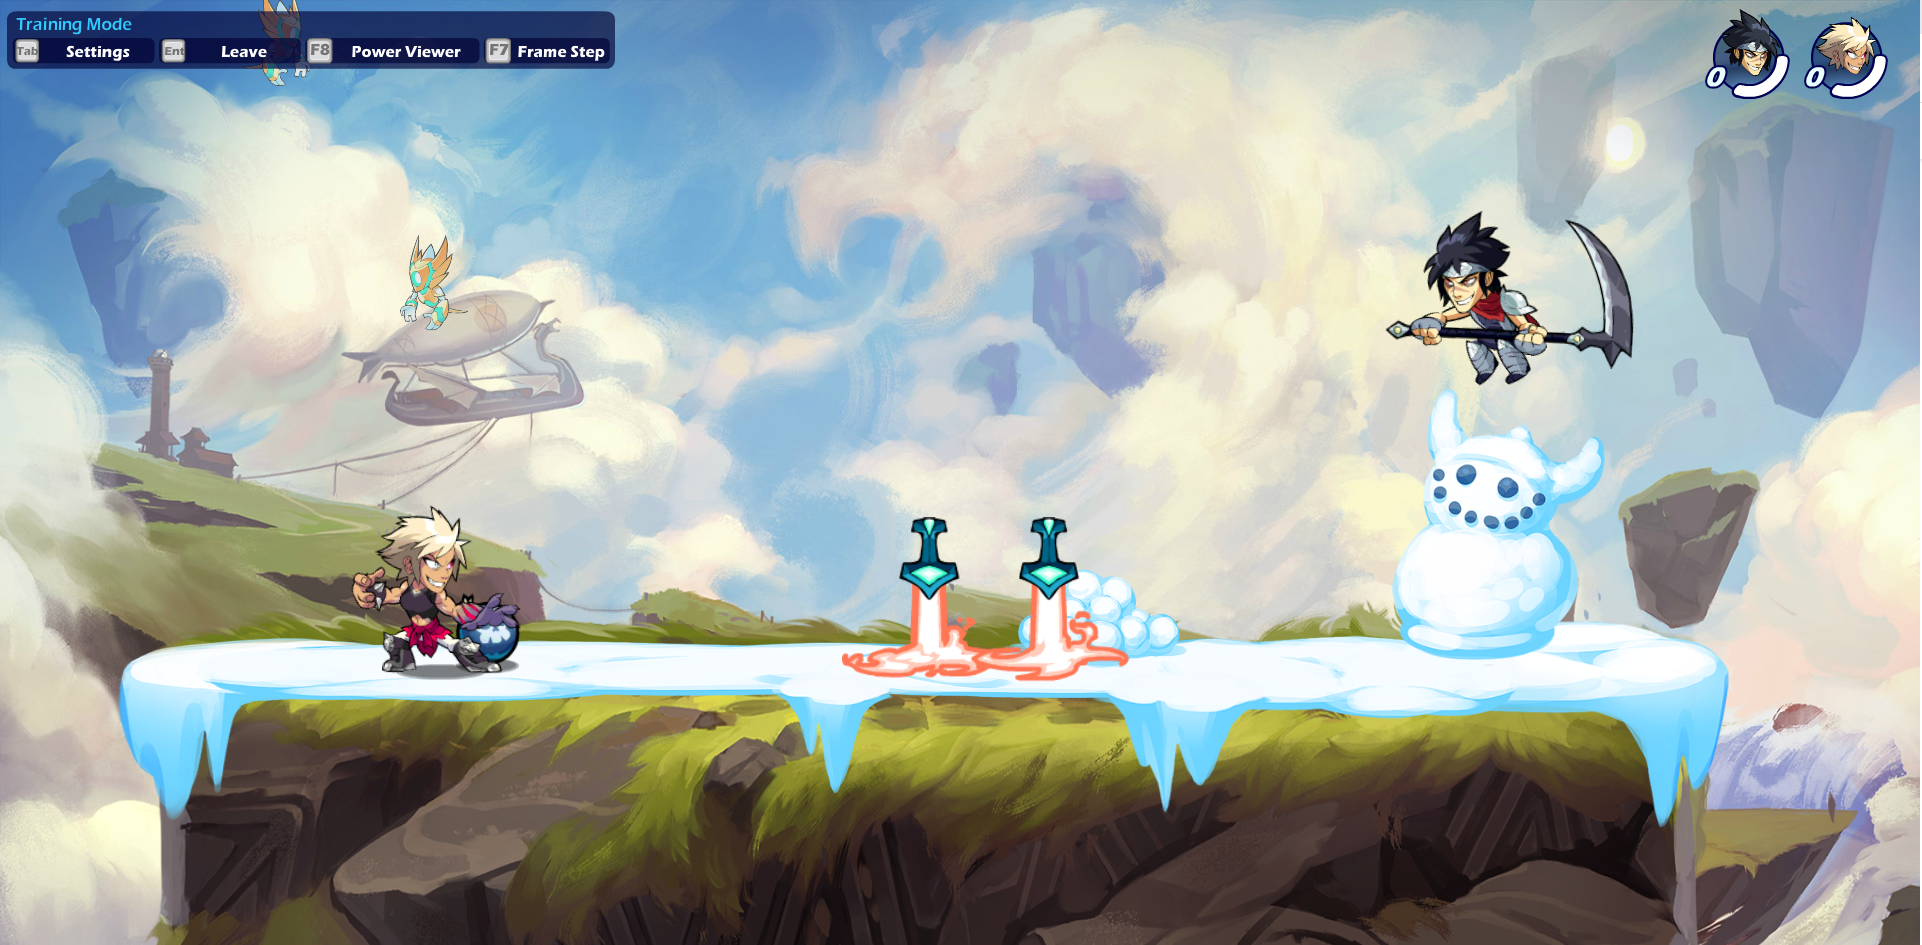
\includegraphics[scale=0.3]{pics/brawlhalla.PNG}

Der Nachteil hierbei ist, dass man sich vor dem Spielen einen Account erstellen
und dann einen Download abschließen muss. Dazu kommt noch, dass man die Spielumgebung nie beeinflussen kann.
Bei Scribble-Fight ist das nicht so. 

\subsection{Stick Fight: The Game}
In dem Spiel Stick Fight kämpft man als Strichmännchen gegeneinander, die durch eine Ragdoll-Engine gesteuert werden.
Auch wie bei schon bei vorher erwähnten Spielen, kann man aber nicht einfach plattformunabhängig im Browser gegeneinander antreten.
Für die Spielekonsole Nintendo Switch zum Beispiel, gibt es das Spiel nicht. Hinzu kommt, dass man auch die Umgebung nicht selbst frei erstellen kann, so wie es bei Scribble-Fight möglich ist.

\section{Ist-Zustand}
Dadurch das es eine Diplomarbeit ist, fängt alles bei 0 an. Es gibt jedoch Frameworks,
welche die Erarbeitung erleichtern. Zum Beispiel im Falle des Spiels, welches
mittels Webtechnologien umgesetzt wird, kann p5.js verwendet werden, welches die
Umsetzung eines Spiels erleichtert. Ein weiteres Beispiel ist die Objekterkennung für
die Spielumgebung (Map). Diese wird von Open-CV übernommen.